\documentclass[a4paper,11pt]{amsart}
\usepackage{epsfig}
\usepackage{fullpage}
\title{Implementing pipeline with embedded farm}
\author{Gagarine Yaikhom}

\begin{document}
\maketitle

We implement the communication structure shown in \mbox{Figure
  \ref{fig:Pipeline Farm}}. There is a farm embedded inside the
pipeline. There are five pipeline stages. The second stage is a farm.

\begin{figure}[htbp]
  \centering
  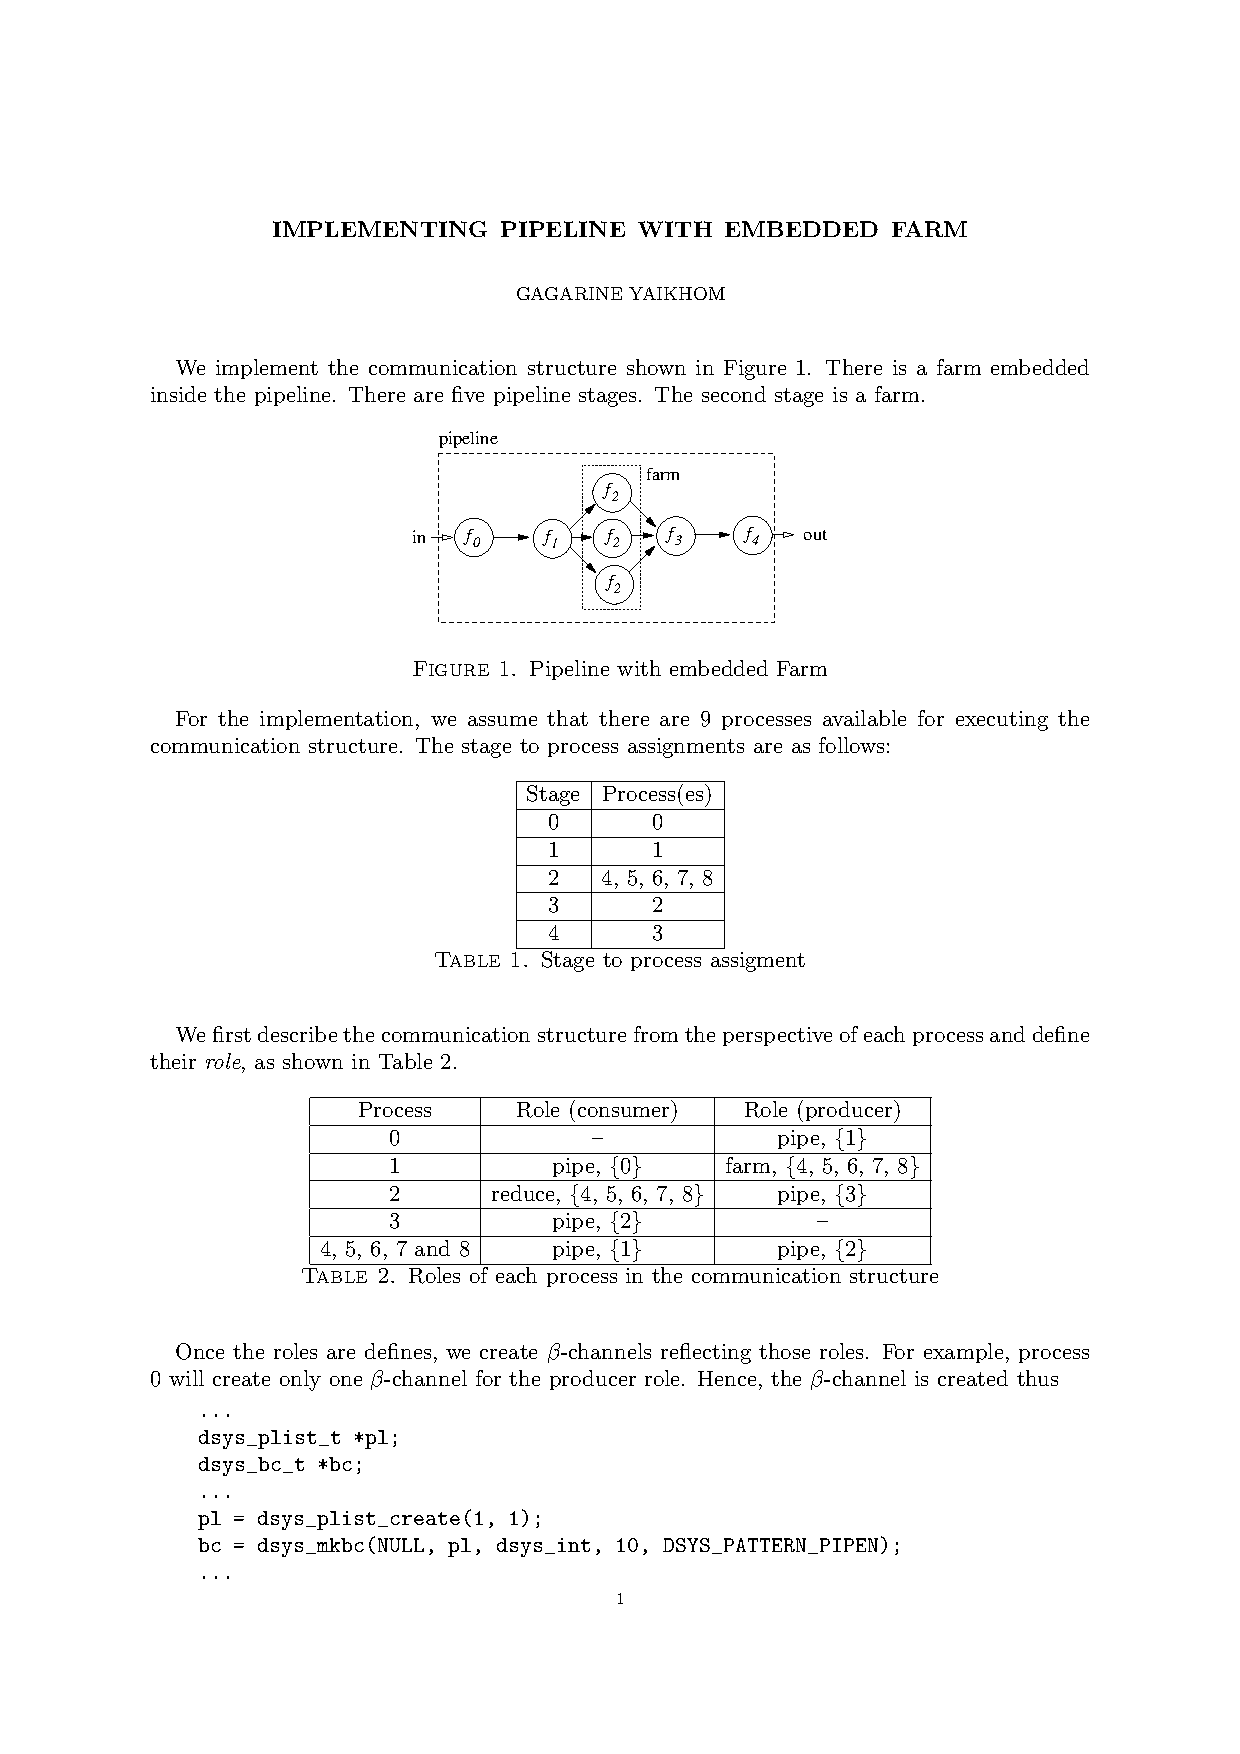
\epsfig{scale=0.7, file=pipeline_farm}
  \caption{Pipeline with embedded Farm}
  \label{fig:Pipeline Farm}
\end{figure}

For the implementation, we assume that there are 9 processes available
for executing the communication structure. The stage to process
assignments are as follows:

\begin{table}[htbp]
  \centering
  \begin{tabular}{|c|c|}
    \hline
    Stage & Process(es) \\  \hline
    0 & 0\\ \hline
    1 & 1\\ \hline
    2 & 4, 5, 6, 7, 8\\ \hline
    3 & 2\\ \hline
    4 & 3\\ \hline
  \end{tabular}
  \caption{Stage to process assigment}
  \label{tab:Stage to Process assignment}
\end{table}

We first describe the communication structure from the perspective of
each process and define their \emph{role}, as shown in \mbox{Table
  \ref{tab:Process Roles}}.

\begin{table}[htbp]
  \centering
  \begin{tabular}{|c|c|c|}
    \hline
    Process & Role (consumer) & Role (producer) \\  \hline
    0 & -- & pipe, \{1\}\\ \hline
    1 & pipe, \{0\} & farm, \{4, 5, 6, 7, 8\}\\ \hline
    2 & reduce, \{4, 5, 6, 7, 8\} & pipe, \{3\}\\ \hline
    3 & pipe, \{2\} & -- \\ \hline
    4, 5, 6, 7 and 8 & pipe, \{1\} & pipe, \{2\}\\ \hline
  \end{tabular}
  \caption{Roles of each process in the communication structure}
  \label{tab:Process Roles}
\end{table}

Once the roles are defines, we create $\beta$-channels reflecting
those roles. For example, process 0 will create only one
$\beta$-channel for the producer role. Hence, the $\beta$-channel is
created thus

\begin{verbatim}
    ...
    dsys_plist_t *pl;
    dsys_bc_t *bc;
    ...
    pl = dsys_plist_create(1, 1);
    bc = dsys_sink_create(pl, dsys_int, 10, DSYS_PATTERN_PIPEN);
    ...
\end{verbatim}

Similarly, process 3 will create only one consumer $\beta$-channel as
follows

\begin{verbatim}
    ...
    dsys_plist_t *pl;
    dsys_bc_t *bc;
    ...
    pl = dsys_plist_create(1, 2);
    bc = dsys_src_create(pl, dsys_int, DSYS_PATTERN_PIPE);
    ...
\end{verbatim}

On the other hand, process 1 will create two $\beta$-channels. One for
consuming data, and the other for producing data. The $\beta$-channels
are created thus:

\begin{verbatim}
    ...
    dsys_plist_t *ipl, *opl;
    dsys_bc_t *ibc, *obc;
    ...
    ipl = dsys_plist_create(1, 2);
    opl = dsys_plist_create(5, 4, 5, 6, 7, 8);
    ibc = dsys_src_create(ipl, NULL, dsys_int, DSYS_PATTERN_PIPE);
    obc = dsys_sink_create(opl, dsys_int, 10, DSYS_PATTERN_FARMN);
    ...
\end{verbatim}

Similarly, we create the other $\beta$-channels. Once this is done,
the communication structure is ready for utilisation. We simply use
these $\beta$-channels as communication handles within the
computation.

\begin{verbatim}
    ...
    loop () {
        dsys_get(ibc, dsys_vptr(obc, int), 1);
        dsys_var(obc, int) += 10;
        dsys_commit(obc);
    }
    ...
\end{verbatim}


Once the process has completed utilising the
communication structure, it can destroy its $\beta$-channels when it
wishes to do so, without actually waiting for the other processes to
complete. We destroy the $\beta$-channels thus:

\begin{verbatim}
    ...
    dsys_bc_destroy(bc);
    dsys_plist_destroy(pl);
    ...
\end{verbatim}

\begin{center}
\textbf{END OF TUTORIAL}
\end{center}

\end{document}
